\documentclass[a4paper, 12pt]{article}
\usepackage{ctex}
\usepackage{amsmath,amscd,amsbsy,amssymb,latexsym,url,bm,amsthm}
\usepackage{epsfig,graphicx,subfigure}
\usepackage{enumitem,balance}
\usepackage{enumerate}
\usepackage{wrapfig}
\usepackage{listings}
\usepackage{mathrsfs,euscript}
\usepackage[usenames]{xcolor}
\usepackage{hyperref}
\usepackage[vlined,ruled,linesnumbered]{algorithm2e}
\hypersetup{colorlinks=true,linkcolor=black}
\lstset{
    breaklines,
    basicstyle          =   \ttfamily,          % 基本代码风格
    commentstyle        =   \rmfamily\itshape,  % 注释的风格,斜体
    stringstyle         =   \ttfamily,  % 字符串风格
    flexiblecolumns,                % 别问为什么,加上这个
    numbers             =   left,   % 行号的位置在左边
    showspaces          =   false,  % 是否显示空格,显示了有点乱,所以不现实了
    numberstyle         =   \zihao{-5}\ttfamily,    % 行号的样式,小五号,tt 等宽字体
    showstringspaces    =   false,
    captionpos          =   t,      % 这段代码的名字所呈现的位置,t指的是top 上面
    frame               =   lrtb,   % 显示边框
}

\newtheorem{theorem}{Theorem}
\newtheorem{lemma}[theorem]{Lemma}
\newtheorem{proposition}[theorem]{Proposition}
\newtheorem{corollary}[theorem]{Corollary}
\newtheorem{exercise}{Exercise}
\newtheorem*{solution}{Solution}
\newtheorem*{example}{Example}
\newtheorem{definition}{Definition}
\theoremstyle{definition}

\renewcommand{\thefootnote}{\fnsymbol{footnote}}

\newcommand{\postscript}[2]
 {\setlength{\epsfxsize}{#2\hsize}
  \centerline{\epsfbox{#1}}}

\renewcommand{\baselinestretch}{1.0}

\setlength{\oddsidemargin}{-0.365in}
\setlength{\evensidemargin}{-0.365in}
\setlength{\topmargin}{-0.3in}
\setlength{\headheight}{0in}
\setlength{\headsep}{0in}
\setlength{\textheight}{10.1in}
\setlength{\textwidth}{7in}
\makeatletter \renewenvironment{proof}[1][Proof] {\par\pushQED{\qed}\normalfont\topsep6\p@\@plus6\p@\relax\trivlist\item[\hskip\labelsep\bfseries#1\@addpunct{.}]\ignorespaces}{\popQED\endtrivlist\@endpefalse} \makeatother
\makeatletter
\renewenvironment{solution}[1][Solution] {\par\pushQED{\qed}\normalfont\topsep6\p@\@plus6\p@\relax\trivlist\item[\hskip\labelsep\bfseries#1\@addpunct{.}]\ignorespaces}{\popQED\endtrivlist\@endpefalse} \makeatother


\title{Install Linux Kernel}
\author{Xuan}
\begin{document}
    \maketitle
    \section{Compile the Linux Kernel}
    \subsection{Preparation}
    We can download and install the \underline{VMWare Workstation Pro 15.5.0}. Then we can download the image file of the Ubuntu operating system \underline{ubuntu-20.04.1-desktop-amd64.iso} from \href{https://mirrors.tuna.tsinghua.edu.cn/}{mirrors.tuna}, and install it as a virtual machine in VMWare Workstation.
    
    After installation, open the terminal of the virtual machine and input the following instruction, and we can see the current Linux Kernel version of the Ubuntu system.

    \begin{lstlisting}
        uname -a
    \end{lstlisting}

    The current Linux Kernel version of my ubuntu is \underline{5.8.0-43-generic} (Fig. \ref{fig1}).

    \begin{figure}[htbp]
        \centering
        % Requires \usepackage{graphicx}
        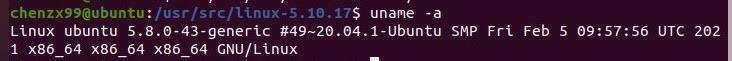
\includegraphics[width=7in]{./pic/exe1/pic1.jpg}\\
        \caption{The current Linux Kernel version}\label{fig1}
    \end{figure}

    Then we can visit the \href{www.kernel.org}{Kernel.org} to download the latest version kernel source. I choose the latest mainline version (\underline{5.11}) to download (Fig. \ref{fig2}).

    \begin{figure}[htbp]
        \centering
        % Requires \usepackage{graphicx}
        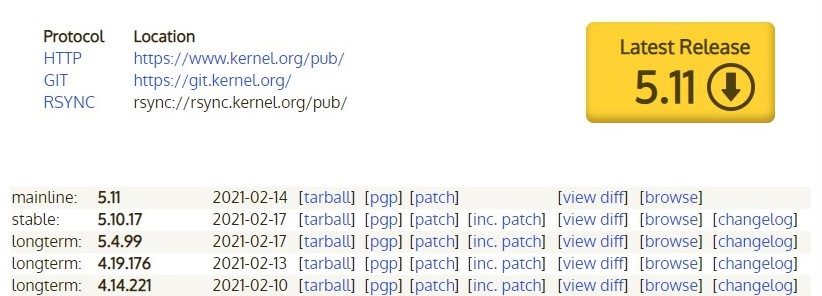
\includegraphics[width=7in]{./pic/exe1/pic2.jpg}\\
        \caption{The latest stable kernel version}\label{fig2}
    \end{figure}

    Then we can use the following instruction to unzip the Linux Kernel source file to the directory \texttt{/usr/src}.

    \begin{lstlisting}
        tar xvJf linux-5.5.8.tar.xz -C /usr/src
    \end{lstlisting}
        
    Before compiling, remember to install or upgrade these tools which is necessary for compilation. Otherwise, sonething would go wrong during compilation.

    \begin{lstlisting}
        sudo apt update
        sudo apt upgrade
        sudo apt-get install build-essential ncurses-dev libssl-dev flex bison
    \end{lstlisting}

    Then, we can use the following instruction to set some configuration of kernel.

    \begin{lstlisting}
        sudo make menuconfig
    \end{lstlisting}

    The configuration menu is displayed as follows (Fig. \ref{fig3}).

    \begin{figure}[htbp]
        \centering
        % Requires \usepackage{graphicx}
        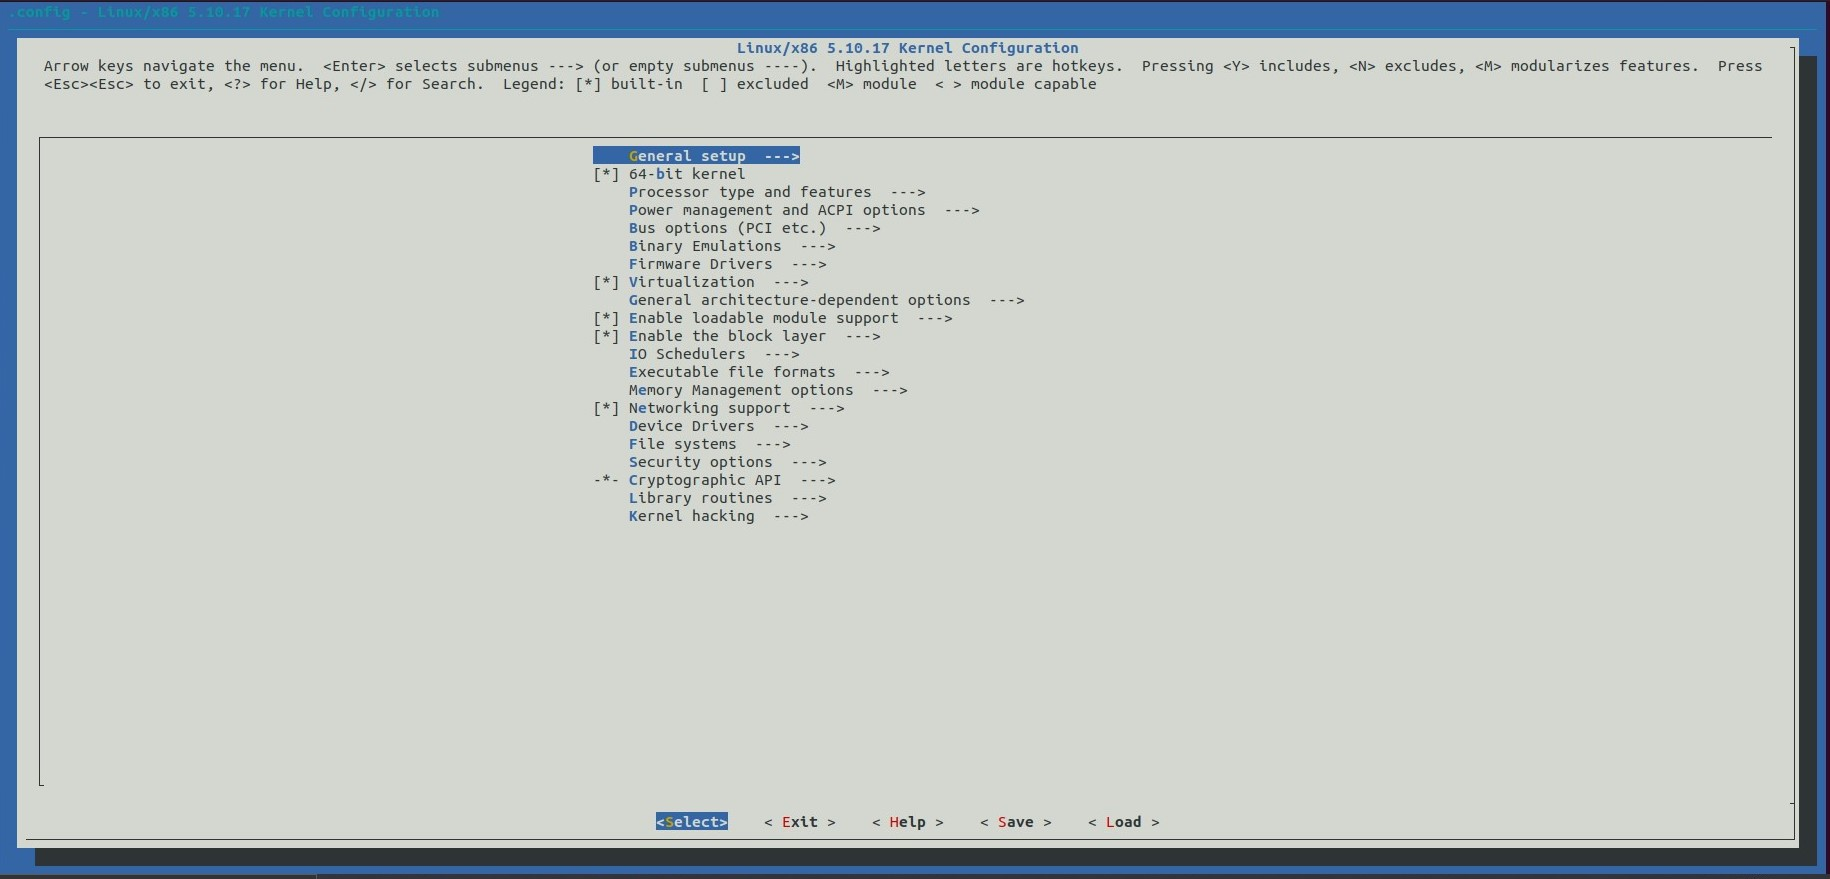
\includegraphics[width=7in]{./pic/exe1/pic3.jpg}\\
        \caption{The configuration menu}\label{fig3}
    \end{figure}

    If there is nothing to be configured, then we can exit directly and the configuration will be saved automatically.

    \subsection{Compilation}
    
    As prompted, we use the following instruction to compile the kernel.

    \begin{lstlisting}
        sudo make
    \end{lstlisting}

\end{document}